\documentclass[10pt]{article}

\usepackage[a4paper,margin=0.65in]{geometry}
\usepackage[utf8]{inputenc}
\usepackage{graphicx}
\usepackage{titlesec}
\usepackage{fancyhdr}
\usepackage{color}
\usepackage{parskip}
\usepackage{helvet}
\usepackage{longtable}
\usepackage{hyperref}
\usepackage{float}
\usepackage{caption}
\usepackage{lastpage}
\usepackage{array}
\usepackage{ragged2e}
\usepackage{makecell}
\usepackage{tabularx}
\usepackage[table]{xcolor}
\usepackage{colortbl}
\usepackage{placeins} % para FloatBarrier

% Colores para tablas
\definecolor{headergray}{gray}{0.9}
\definecolor{rowalt}{RGB}{245,245,255}

% Fuente sans-serif
\renewcommand{\familydefault}{\sfdefault}

% Encabezado
\pagestyle{fancy}
\fancyhf{}
\lhead{
\includegraphics[height=0.7cm]{images/logo_unit.png}}
\rhead{\textbf{CN3165 battery charger module v1.0}}
\lfoot{Product Brief}
\rfoot{\thepage\ | \pageref{LastPage}}

% Estilo de secciones
\titleformat{\section}{\bfseries\large\sffamily}{}{0em}{}
\titleformat{\subsection}{\bfseries\normalsize\sffamily}{}{0em}{}
\titlespacing*{\section}{0pt}{1.2em}{0.5em}
\titlespacing*{\subsection}{0pt}{0.8em}{0.4em}

\title{}
\author{}
\date{}

\sloppy
\setlength{\emergencystretch}{3em}

\begin{document}

% Encabezado del documento
\noindent
\makebox[\textwidth][l]{%
    \begin{minipage}[t]{\textwidth}
        \Large \textbf{CN3165 battery charger module Product Brief}\\[1.0em]
        \normalsize This compact printed circuit board functions as both a single-cell Li-Ion battery charger and a power-out module\\[0.3em]
        \footnotesize\textsf{Version: 1.0 \hfill Modified: 2025-05-02}
    \end{minipage}%
}
\vspace{1em}
\hrule
\vspace{1.5em}

% Introducción con imagen
\section*{Introduction}
\vspace{0.5em}
\noindent
\begin{minipage}[t]{0.62\textwidth}
\setlength{\parskip}{0.75em}
\justifying
This compact printed circuit board functions as both a single-cell Li-Ion battery charger and a power-out module. It features a USB-C interface that accepts a stable 5 V supply from sources such as PCs, charger bricks, or power banks, and includes an on-board charger IC that supports charging currents of 250 mA, 750 mA, or 1 A. Additionally, two dedicated screw-terminal outputs provide a secure pathway for charging (Battery In) and deliver battery voltage to a load even during charging (Battery Out), making it suitable for portable applications that demand simultaneous charging and power delivery.
\end{minipage}
\hfill
\begin{minipage}[t]{0.35\textwidth}
\centering
\vspace{-0.5em}
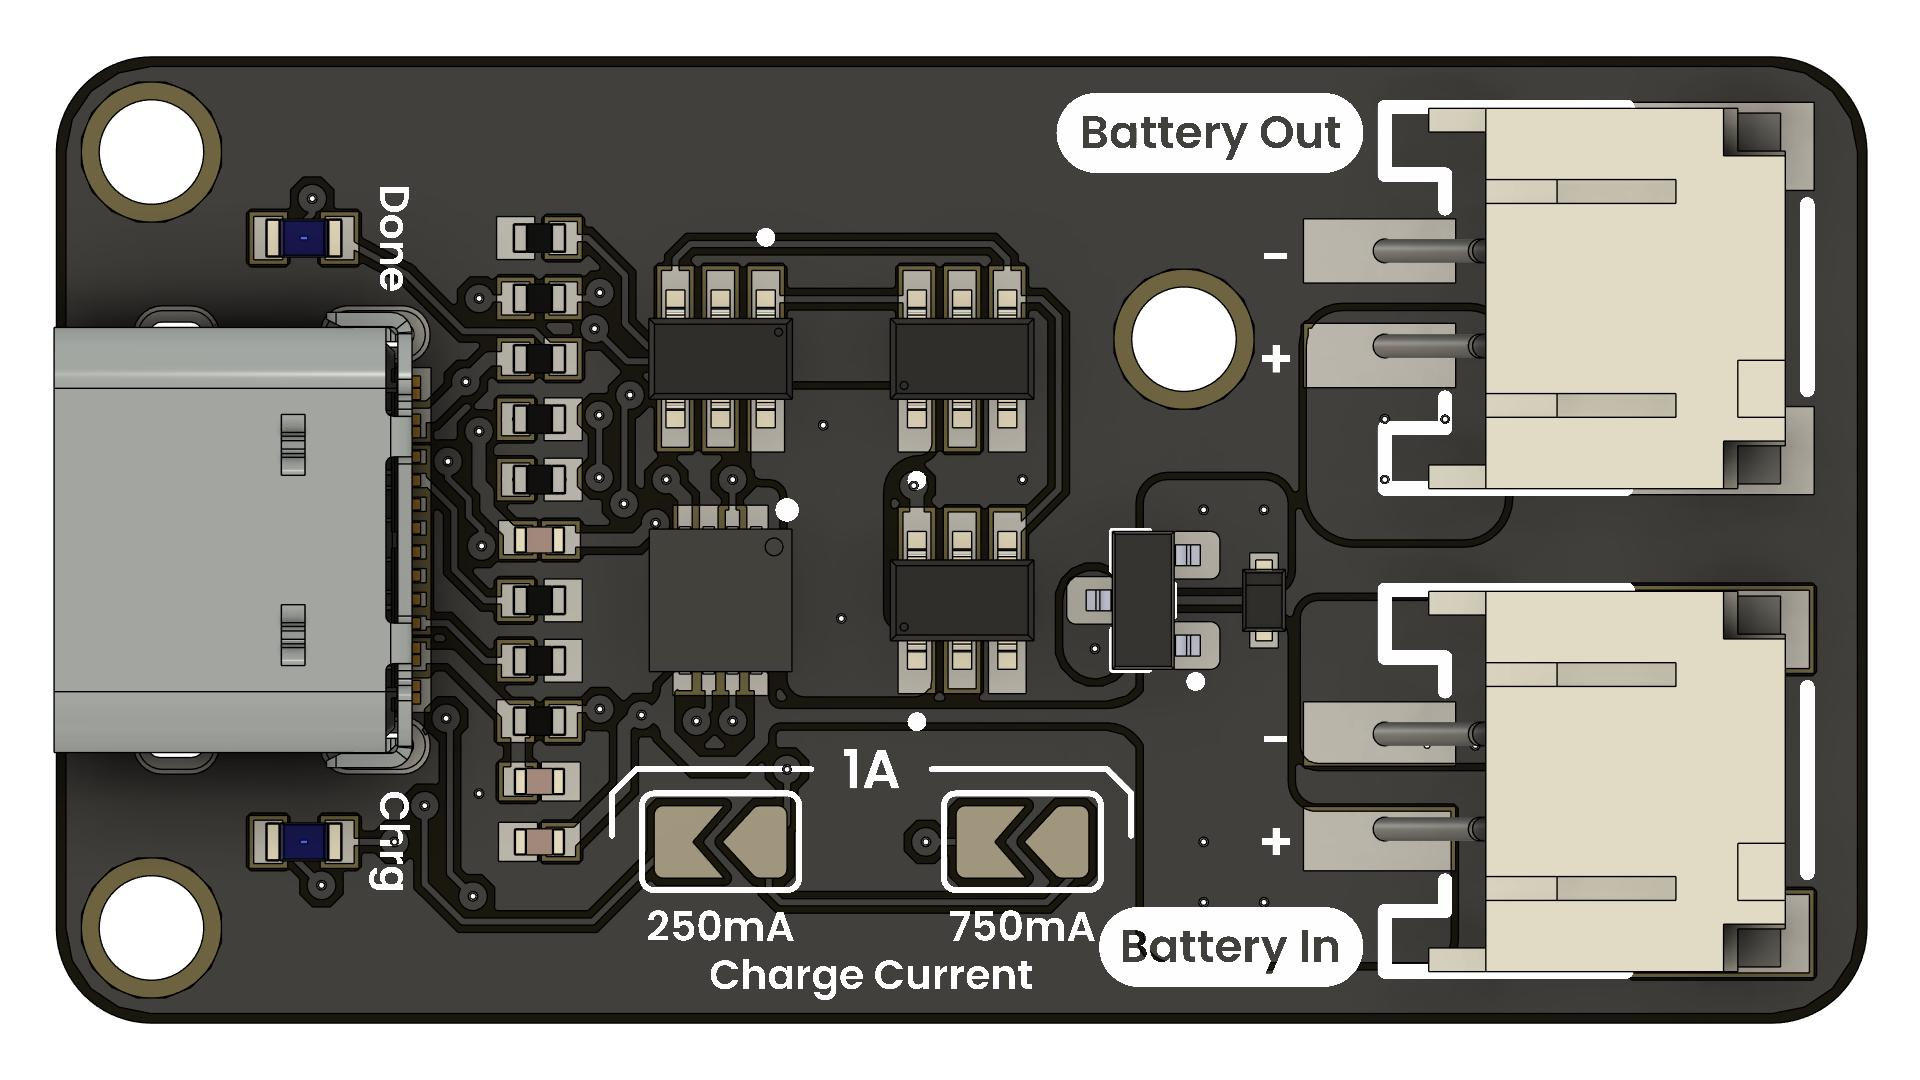
\includegraphics[height=4.5cm,keepaspectratio]{./images/product.jpg}
\end{minipage}

\vspace{1.0em}
\FloatBarrier % evita que la imagen flote sobre el siguiente bloque



% Secciones técnicas
\section*{Functional Description}
- The USB-C port accepts a 5 V supply from PCs, charger bricks, or power banks.\\ 

\section*{Electrical Characteristics}
- **Input Voltage:** 5 V (USB-C)\\ 

\section*{Features}
- USB-C power input\\ 



\section*{Applications}
- Battery charger for single-cell Li-Ion batteries\\ 
- Power supply for low-power devices\\ 

\vspace{1em}



\section*{Settings}

\subsection*{Interface Overview}
\rowcolors{2}{white}{rowalt}
\begin{tabularx}{\textwidth}{|c|c|>{\RaggedRight\arraybackslash}X|}
\hline
\rowcolor{headergray}
Interface & Signals / Pins & Typical Use \\
\hline
- & - & - \\
\hline
\end{tabularx}


\subsection*{Supported Pins}
\rowcolors{2}{white}{rowalt}
\begin{tabularx}{\textwidth}{|c|c|>{\RaggedRight\arraybackslash}X|}
\hline
\rowcolor{headergray}
Symbol & I/O & Description \\
\hline
- & - & - \\
\hline
\end{tabularx}




% Tabla principal
\section*{Pin \& Connector Layout}
\rowcolors{2}{white}{rowalt}
\begin{tabularx}{\textwidth}{|c|c|>{\RaggedRight\arraybackslash}X|}
\hline
\rowcolor{headergray}
Component & PCB Label & Description \\
\hline
USB-C Connector & USB IN & 5 V power input from USB-C source \\
Connector & Battery IN & Screw terminals for connecting the Li-ion cell \\
Connector & Battery Out & Screw terminals for outputting battery voltage \\
CHRG LED & CHRG & Indicator LED: on during the charging phase \\
DONE LED & DONE & Indicator LED: on when the charging cycle completes \\
\hline
\end{tabularx}


% Imágenes adicionales
\FloatBarrier
\newpage
\vspace*{3em}
\section*{Block Diagram}
\vspace{1em}
\begin{center}
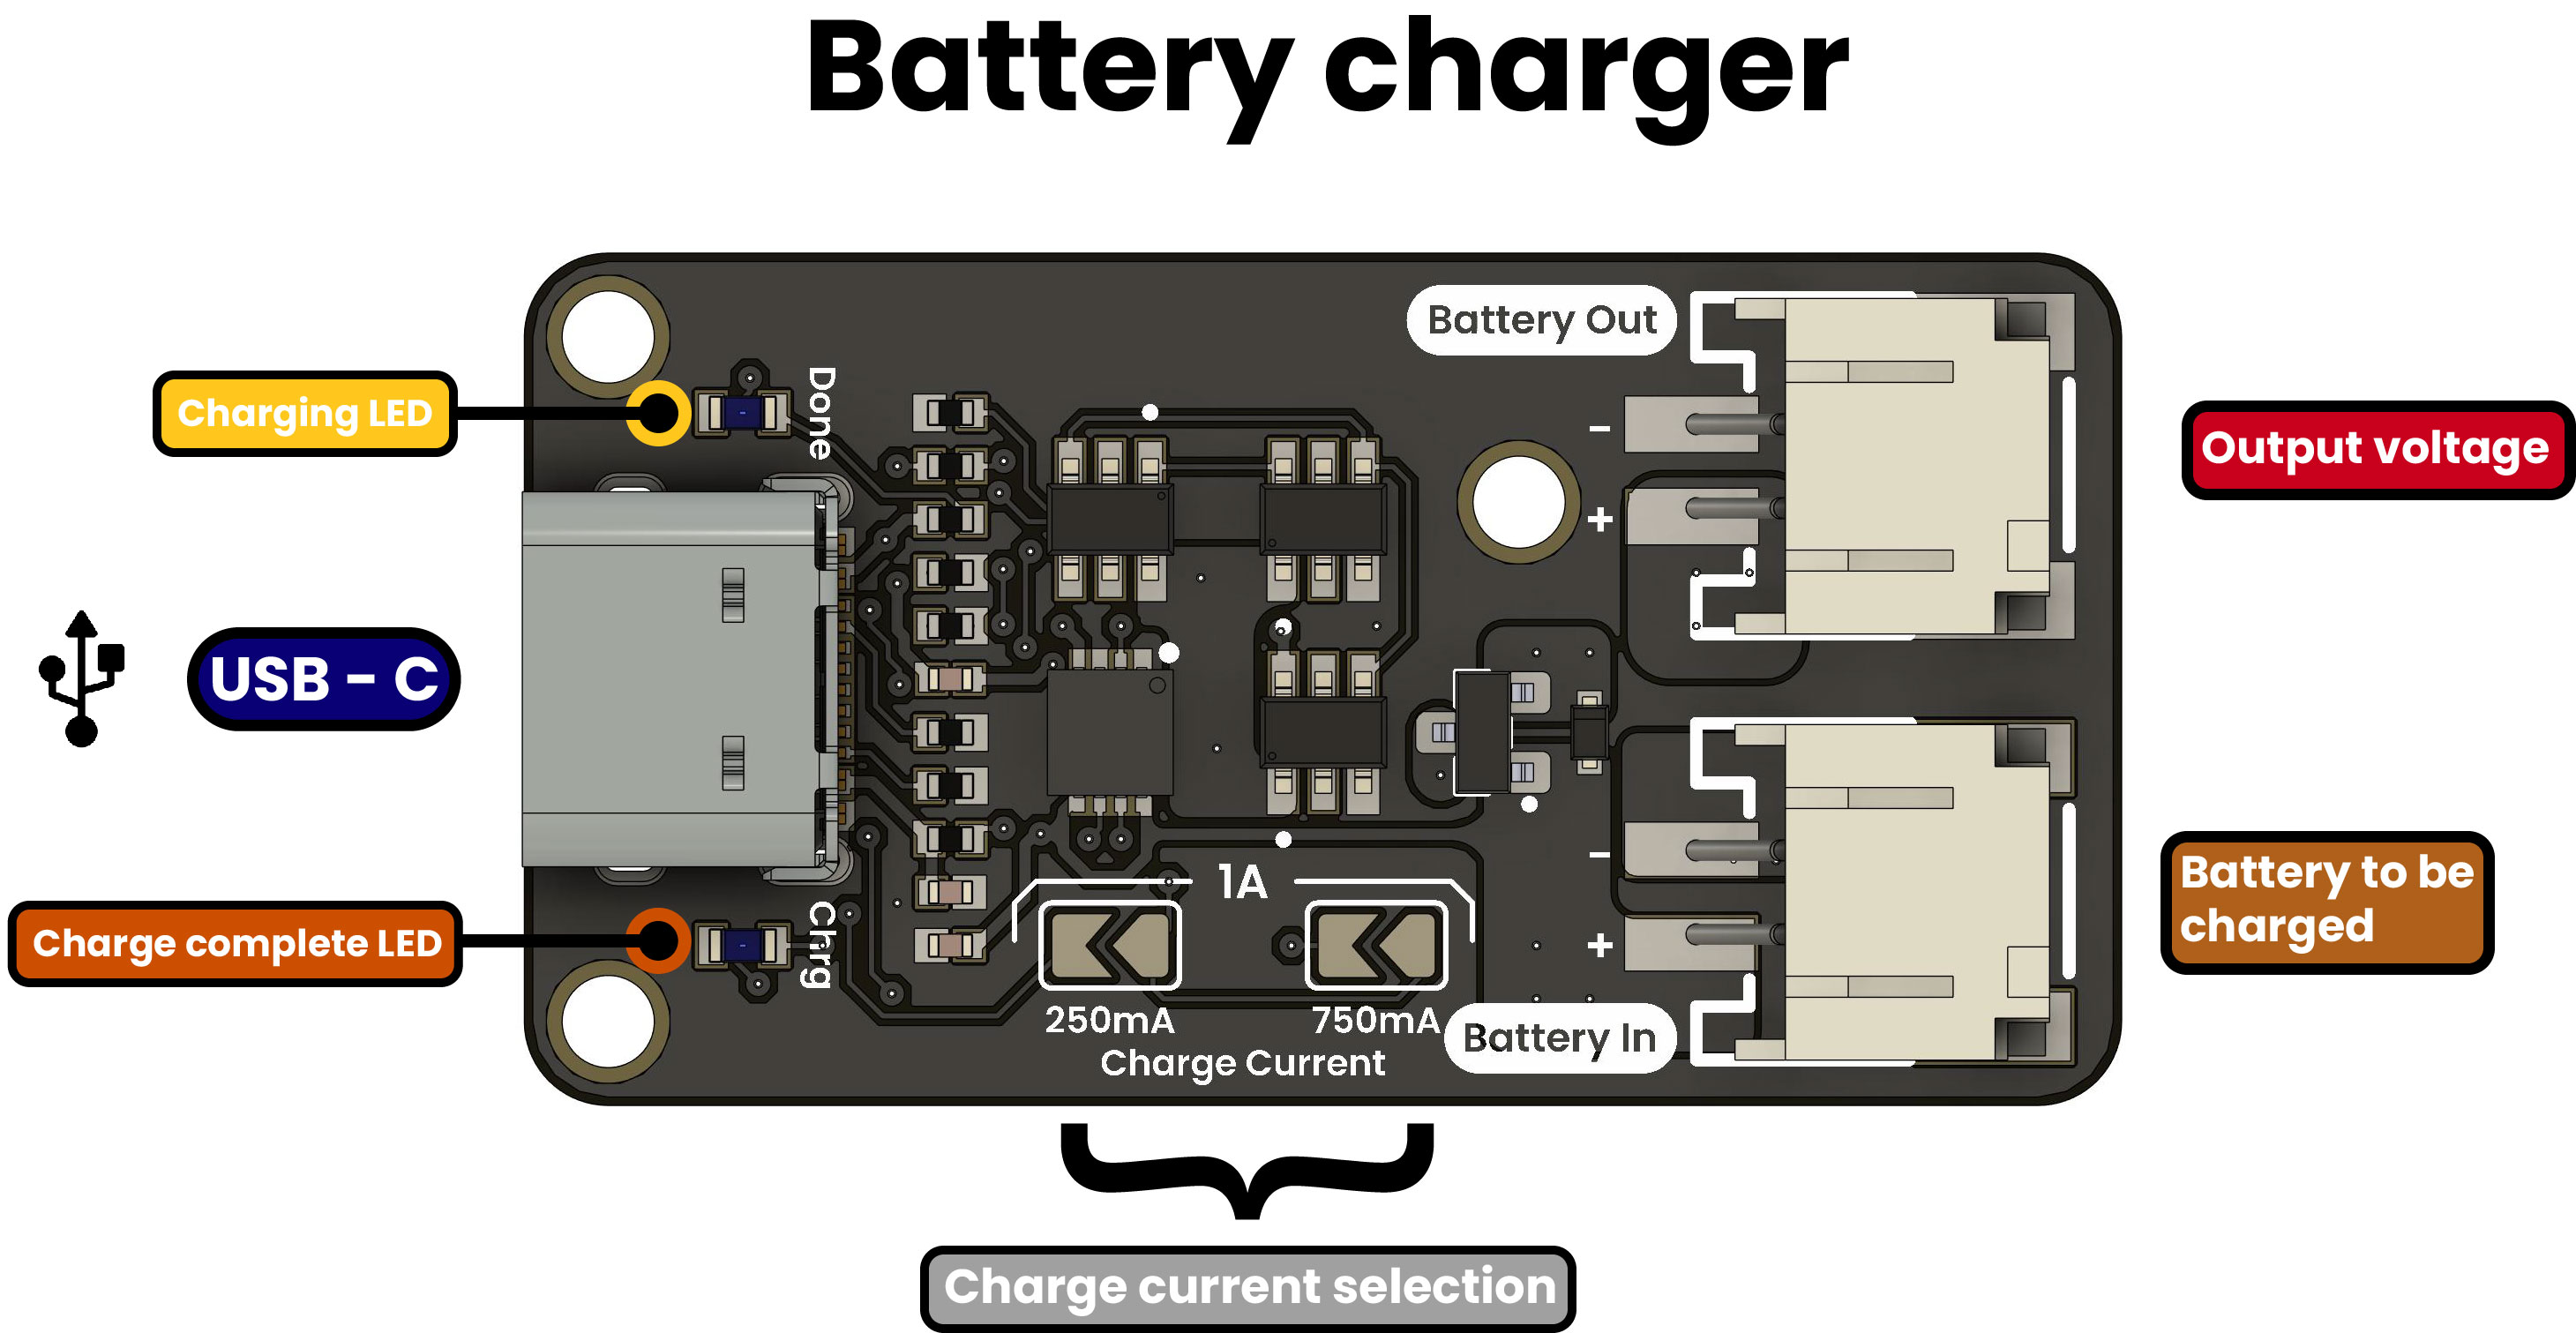
\includegraphics[width=0.95\textwidth,keepaspectratio]{images/function-diagram.jpg}
\end{center}
\newpage
\vspace*{3em}
\section*{Dimensions}
\vspace{1em}
\begin{center}
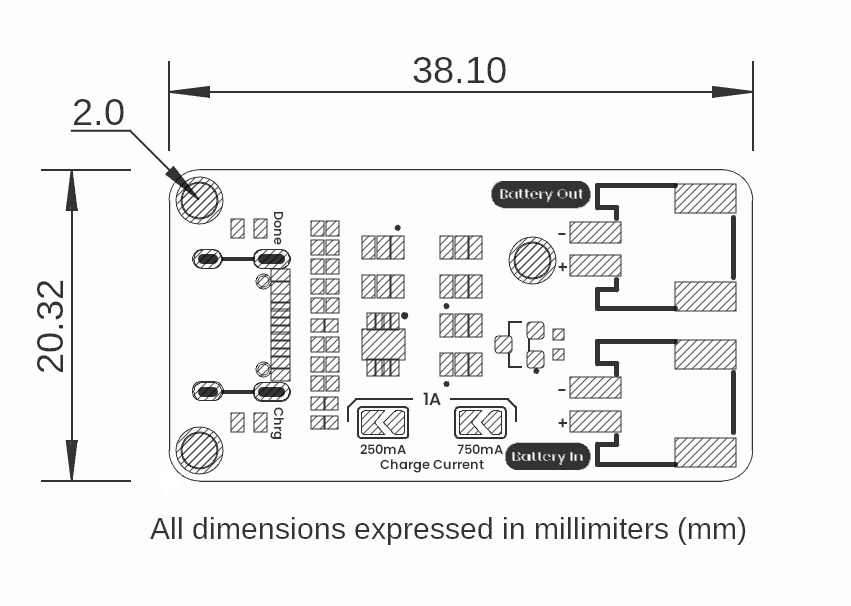
\includegraphics[width=0.95\textwidth,keepaspectratio]{images/dimensions.png}
\end{center}



% Uso
\section*{Usage}
\begin{itemize}
\item 
\end{itemize}

% Descargas
\section*{Downloads}
\begin{itemize}
\begin{itemize}
\item \href{docs/schematic.pdf}{Schematic PDF}
\end{itemize}
\end{itemize}

% Compra
\section*{Purchase}
\begin{itemize}
\item \href{https://www.uelectronics.com}{Buy from UNIT Electronics}
\end{itemize}

\end{document}
